% Chapter 1

\chapter{Methodology} % Write in your own chapter title
\label{Chapter4}
\lhead{Chapter 4. \emph{Methodology}} 
\section{Overview}

IP Cameras were wall mounted in the room of the patient for visual input. The video stream is sent at desktop application via an internet connection. Here the activity recognition algorithms namely, the Boundary Sensitive Network (BSN) and Temporal Segment Network (TSN) work in tandem to recognize the activity of the person. The Activity logs generated from these algorithms were then sent to a Django backend via HiveMQTT and Pusher Websockets. This double setup allows for higher throughput. 
\begin{figure}[H]
    \centering
    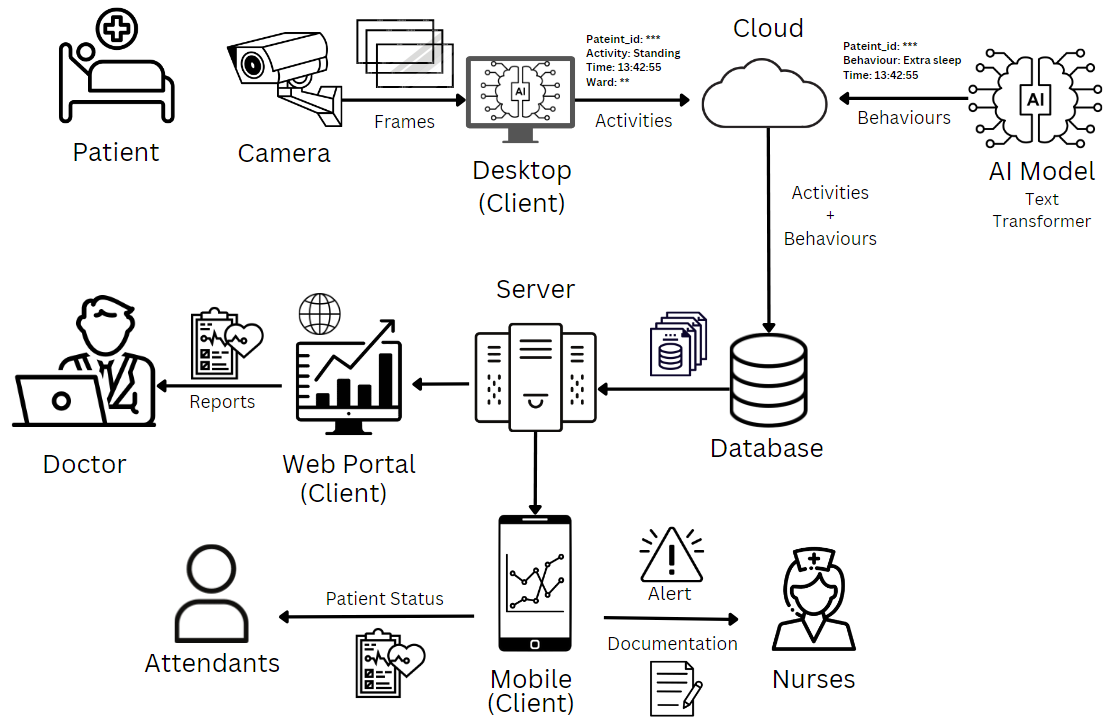
\includegraphics[width=0.8\textwidth]{images/arch.png}
    \caption{Project Process Flow}
    \label{fig:mesh1}
\end{figure}
The activities are stored in the InfluxDb Cloud and  processed by a time series text transformer to forecast patient activities. The admin on the other creates an account and sets up Doctors, Nurses and Patients on the web portal developed in ReactJs. The portal uses HTTPs connections to establish a secure connection with the Django Web app. It authenticates and authorizes each user before allowing access to any requested resources. The dashboard shows the patient's next forecast activity from the current logs. An API call to a web app responds to the user with patient logs in tabular form and Gemini's analytical response to any prompt from the user. When a reading has been missing for more than an hour or  unidentified consumption is perceived, Firebase is used to send push notifications to nurses to prompt  manual logging. The patient's attendants and relatives may also login via patient credentials on the mobile app to check the patient's status remotely. The overall data flow is shown in figure \ref{fig:mesh1}
\begin{figure}[H]
    \centering
    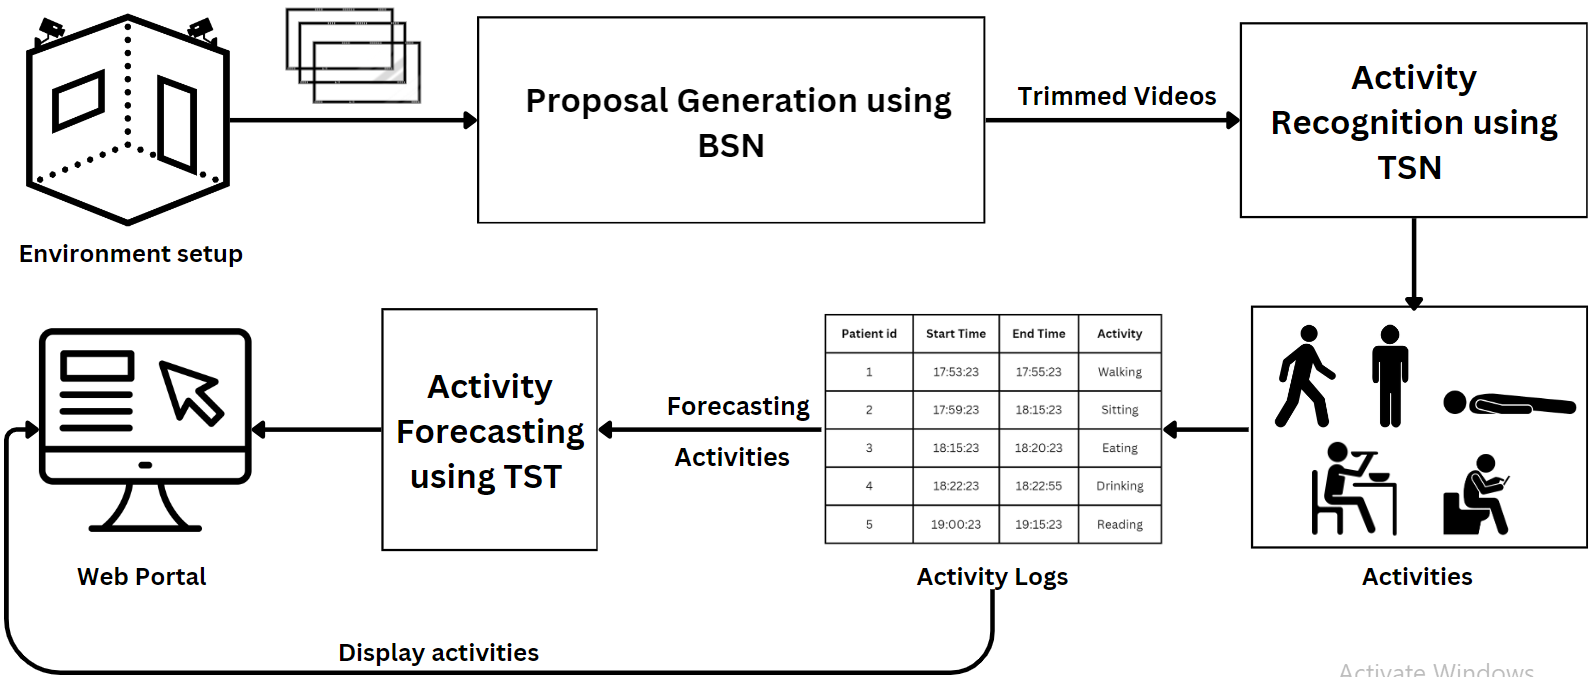
\includegraphics[width=\textwidth]{images/archdia.png}
    \caption{High Level Architecture}
    \label{fig:level 0 diagram}
\end{figure}
At the algorithmic level, figure \ref{fig:level 0 diagram} shows how the video stream is converted to useful information for the doctor. The frames received from the environment are first passed to the BSN for activity localization. The model generates proposals for the incoming video which is then sent to the TSN model. These proposals define the duration in which certain activities have occurred. The TSN model uses these proposals to extract a portion of the video and recognize the activity from the video. Once the current frames are recognized, the subsequent incoming frames are processed. The textual logs generated are then displayed on the web portal and  used to forecast patient activity which is also displayed to the user.

\section{Activity Recognition}
        To understand the purpose of each algorithm better, the types of algorithms must be explained prior to any in-depth dive into a concept. When a person moves a leg it becomes an action which can be labeled as "moving leg". Combining multiple actions such as moving both legs one after another makes an activity which can then be labeled as "walking". Once an activity is performed over a longer duration, it becomes a behavior and generates patterns that can be analyzed. Recognition refers to the identification type of anything. The problem of action recognition and activity recognition has long been solved on trimmed data where videos are small clips of not more than 10 s where an activity starts at the beginning of the clip and ends at the end of the clip. When we pass untrimmed videos or  video streams, we introduce two problems. Activity Detection and Localization. Detection refers to whether an activity is occuring. Localization refers to the identification of the time period during which an activity occurs. After these first two problems are solved, only action recognition, which is a process of classifying and labelling an activity can be processed. 
\begin{figure}[H]
    \centering
    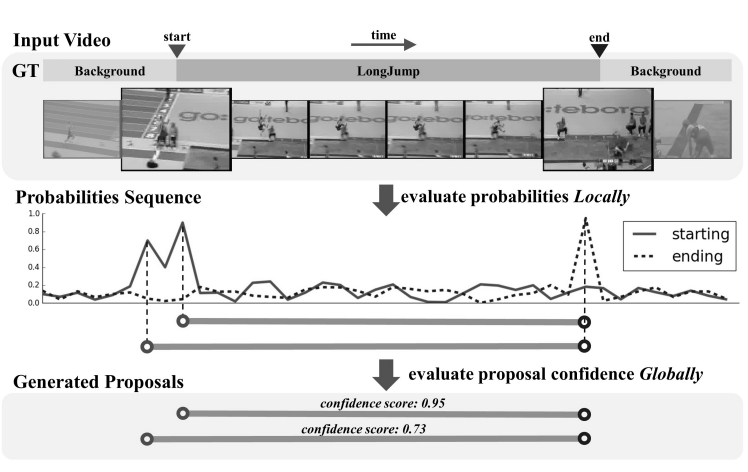
\includegraphics[width=\textwidth]{images/overviewBSN-modified.png}
    \caption{Overview of BSN}
    \label{fig:bsn overview}
\end{figure}
        A boundary sensitive network is used for temporal action proposal generation as shown in figure \ref{fig:bsn overview}. This process is divided into two parts. The first part contains temporal action detection, where the objective is to identify the action areas within the untrimmed videos. This section also provides temporal boundaries and action classes. This step allows for the detection of actions areas throughout the entire video. The second part of the process contains the classification of the action areas identified by the first part of the video stream, each containing a single action. By combining these two components, the methodology provides an approach to action proposal generation. 

\subsection{Properties of proposals}
\begin{itemize}
    
    \item  The proposed system should be capable of capturing actual action instances without generating numerous proposals. 
    \item  The system should also be capable of achieving accurate temporal alignment with ground truth action instances while generating a minimum number of proposals.Thus, the computational cost is reduced because fewer proposals require fewer resources.
\end{itemize}

\subsection{Problem Definition}
The untrimmed video sequence is represented as:
\begin{equation}
X = \{x_n\}^{\text{lv}}_{n=1}
\end{equation}
where, lv is the total number of frames. \(x_n\) is the nth frame in \(X\). Annotation of untrimmed video \(X\) is contained in a set of action instances 
\begin{equation}
    \Psi_g = \{\phi_n = (t_{s,n}, t_{e,n})\}^{N_g}_{n=1}
\end{equation}
where \(N_g\) is the total number of true action instances in a given video sequence \(X\). The starting and ending times of the action instances were \(t_{s,n}\) and \(t_{e,n}\), respectively. The set of annotation \(\Psi_g\) is used during the training process. During the prediction, the set of predicted annotations \(\Psi_p\) should cover \(\Psi_g\) with high precision.
\subsection{Video Features Encoding}

The two-stream network is  divided into two branches:  spatial  and  temporal networks. The spatial network is used to recognize the appearance features of objects and it operates step-by-step on a single RGB frame. In contrast, a temporal network focuses on extracting motion information by working with stacked optical flow fields as shown in figure \ref {fig:encoding-of-vedio-features}. 
\begin{figure}[H]
    \centering
    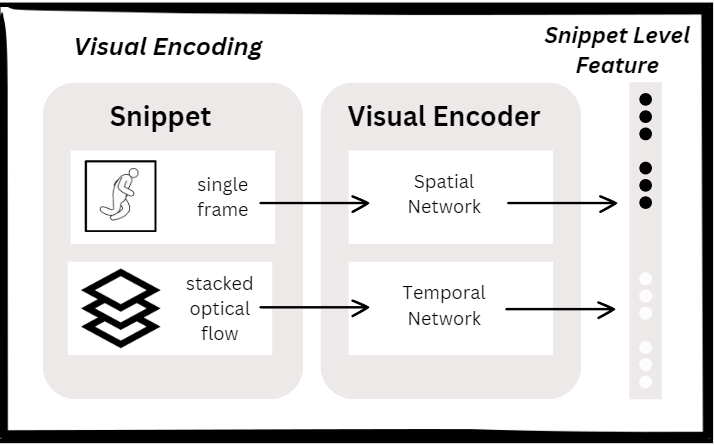
\includegraphics[width=0.7\linewidth]{images/ti1.png}
    \caption{Encoding of Video Features}
    \label{fig:encoding-of-vedio-features}
\end{figure}
This illustrates the movement between different frames. The output scores from both networks are then combined to create an encoded feature vector for each snippet. This vector, concatenates the spatial and temporal network outputs for all the snippets in the dataset. These two-stream feature sequences are very important, because they serve as inputs for the  Bounding Box Selection of the methodology. The integration of spatial and temporal information enhances the overall understanding and analysis of the video data.
Mathematically, the snippet sequence of  vedio is represented as:
\begin{equation}
    S = \{s_n\}^{\text{ls}}_{n=1}
\end{equation}
Here, the length of snippets sequence is represented as ls.
\begin{equation}
    s_n = (x_{t,n}, o_{t,n})
\end{equation}
The snippet above contains two parts. The first part  \(x_{t,n}\) is the spatial network. Here, \(x_{t,n}\) is the \(t_n-th\) RGB frame in Video X. It is used to recognize the appearance features of an object in a video. By contrast,  \(o_{t,n}\) focuses on extracting motion information by working with stacked optical flow fields. Snippets after a regular frame interval are:
\begin{equation}
    ls = \frac{lv}{\sigma}
\end{equation}
We concatenated the output of the spatial and temporal networks to form the encoded feature vector. This vector is represented as:
\begin{equation}
    ftn = (fS_{t,n}, fT_{t,n})
\end{equation}
Here,\(fS_{t,n}\) and  \(fT_{t,n}\) are the outputs of the spatial and temporal processes respectively, for all the snippets, the feature vector is represented as:
\begin{equation*}
    F = \{ftn\}^{ls}_{n=1}
\end{equation*}
This feature vector is used as an input to BSN.

\subsection{Temporal evaluation module}
The temporal evaluation module was used to evaluate the probabilities of the starting, ending, and actionness of events at all  temporal locations. This module uses three temporal convolutional layers to obtain temporal features from the input data. Notably, the first two layers use rectified linear unit (ReLU) activation functions, whereas the third layer uses the sigmoid activation function, which is used  to generate probability values as shown in \ref {fig:tem}. The results of this temporal evaluation module contained three probability sequences. This approach integrates an advanced convolutional neural network architecture to capture meaningful insights from the given input.
\begin{equation}
    \text{Conv}(512, 3, \text{Relu}) \rightarrow \text{Conv}(512, 3, \text{Relu}) \rightarrow \text{Conv}(3, 1, \text{Sigmoid})
\end{equation}

The first two layers use ReLU activation, whereas the last one uses  the sigmoid activation function.The feature sequence was divided into non-overlapping windows for the input of the temporal evaluation module.The temporal evaluation module generates the following three probabilities: 

\begin{equation}
    PS = \{p_{s,t_n}^{ls}\}_{n=1}, \quad PE = \{p_{e,t_n}^{ls}\}_{n=1}, \quad PA = \{p_{a,t_n}^{ls}\}_{n=1}
\end{equation}

Above three are starting, ending and actionness probabilities respectively.

\begin{figure}[h]
    \centering
    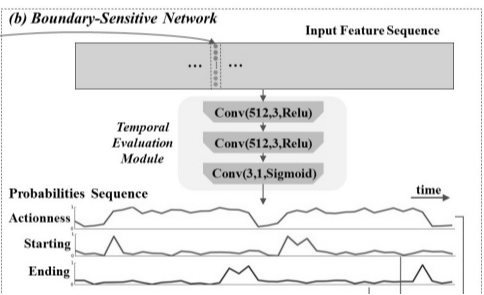
\includegraphics[width=0.8\linewidth]{images/tem2a.png}
    \caption{Temporal Evaluation Module}
    \label{fig:tem}
\end{figure}

\subsection{Proposal generation module}
The main purpose of the proposed generation module is to create proposals for the most important regions of interest in a given video. For this purpose, we followed 2 steps. First, we   identified  time intervals with very high boundary probabilities. These boundaries were then used to define the starting and ending points of the proposals. In the second step, we combine the identified intervals to form complete proposals. We created a Boundary-Sensitive Proposal (BSP) feature for each proposal as shown in figure \ref {fig:gp}. This allowed us to  generate effective proposals for further analysis. 
Initially all  the temporal locations \(t_n\) are recorded, where the staring probabilities \(p^{s}_{t_n}\) are very high. Let say: 
\begin{equation}
    (p^{s}_{t_n}) > 0.9 
\end{equation}
Or starting probability is a peak of that particular region
\begin{equation}
    p_{s,t_n} > p_{s,t_{n-1}} \quad \text{and} \quad p_{s,t_n} > p_{s,t_{n+1}} 
\end{equation}  
These locations are grouped to form a set of candidate starting locations \(B_S = \{ts_i\}_{i=1}^{NS}\) where \(N_S\) represents the total number of candidate starting locations. The same procedure is followed for the generation of the candidate ending location set \(B_E\). Subsequently, we generated temporal regions by combining every starting location with each ending location. As a result, we obtain the candidate proposal set:
\begin{equation}
    \Psi_p = \{\phi_i\}_{i=1}^{N_p}
\end{equation}
where \(N_p\) is the total number of proposals. For each candidate proposal, its center region is denoted by \(r_C\) and its starting and ending regions are denoted by \(r_S\) and \(r_E\) respectively. 
\begin{figure}[h]
    \centering
    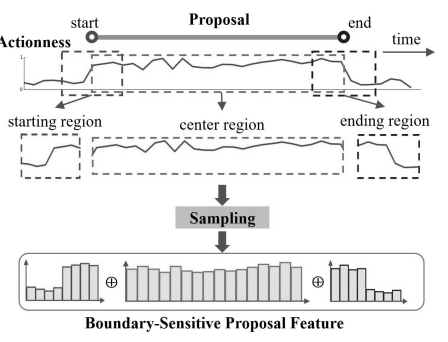
\includegraphics[width=0.7\linewidth]{images/BSPFeature-modified.png}
    \caption{Generating Proposals}
    \label{fig:gp}
\end{figure}
The action sequence within the center region is then represented by \(f^{A}{c}\). It was formed by linearly interpolating the 16 points. On the other hand, the action sequence within the starting and ending regions is represented by \(f^{A}{s}\)  and \(f^{A}{e}\) respectively by linearly interpolating eight points after which a BSP feature is formed.
\begin{equation}
    \mathbf{f_{BSP}} = (f_A^s, f_A^c, f_A^e)
\end{equation}
then every proposal is represented as:
\begin{equation}
    \phi = (ts, te, \mathbf{f_{BSP}})
\end{equation}
\subsection{Proposal evaluation module}
The main objective of the proposed evaluation module was to assign a confidence score to each proposal. This determines whether the actionness instance occurs during the duration. To achieve this, a simple multilayer model was used. It contained a single hidden layer of 512 units. This layer used a Rectified Linear Unit (Relu) activation function. The output layer uses  sigmoid activation to generate the confidence score. This  architecture enables an effective evaluation of action presence within the proposed time as shown in figure \ref {fig:pem}. 


Mathematically,
\begin{equation}
    \phi = (ts, te, \text{pconf}, p_{s_{ts}}, p_{e_{te}})
\end{equation}
where \(p_{s_{ts}}\) and \(p_{e_{te}}\) are the staring and ending probabilities, respectively \(t_s\) and \(t_e\) are the start and end time locations, respectively and \text{pconf} is the confidence score.
\begin{figure}
    \centering
    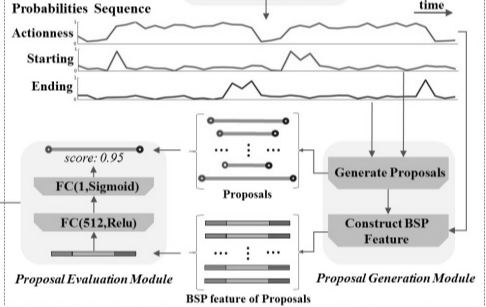
\includegraphics[width=0.7\linewidth]{images/proposalEvaluation-modified.png}
    \caption{Generating Evaluation}
    \label{fig:pem}
\end{figure}


\section{Time series transformer for representation learning}
Time series forecasting is a critical task in various domains, ranging from finance and climate science to the healthcare sector. Traditional methods including the use of Recurrent Neural Networks (RNN) and Convolutional Neural Networks (CNN) face challenges in capturing long-term dependencies in sequential data. On the other hand, transformers keep a connection to all previous timestamps and data, which allows information to propagate over longer sequences. This brings forward the problem of handling large input which is then taken care of by filtering important and unimportant data using the technique of self-attention.
\subsection{Transformer}
Transformer architecture is used under the hood for forecasting methodology, hence it is important to understand how it operates to fully comprehend how forecasting is performed. The transformer is divided into two main components: \textbf{Encoder} and \textbf{Decoder}.
The encoder part as shown in figure \ref{fig:encoder} of the transformer works on the input and it's output is then used in the decoder to process the output. This is done in multiple passes and unlike a feed-forward network, there is only forward propagation and no backward propagation involved in a transformer.
\begin{figure}[h]
    \centering
    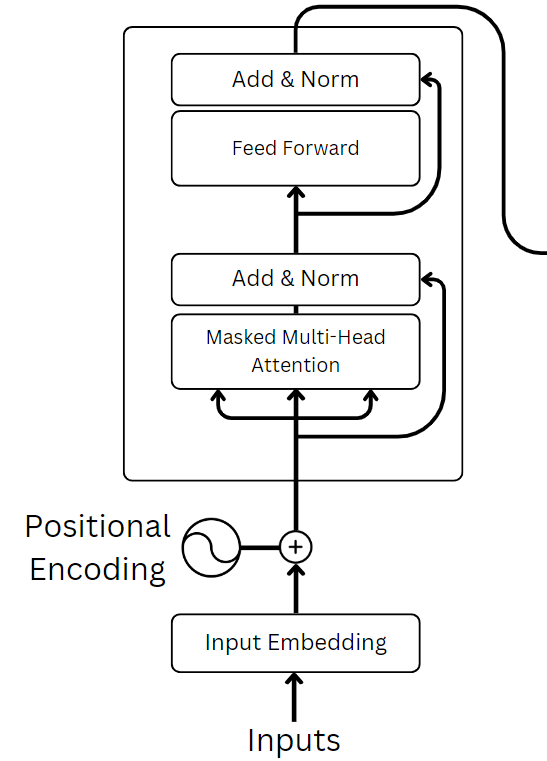
\includegraphics[width=0.35\textwidth]{images/encoder.png}
    \caption{Encoder of a Transformer}
    \label{fig:encoder}
\end{figure}
\subsubsection{Input processing}
The data passed to the transformer is in textual form. A token is not exactly equivalent to a word but for the sake of understanding can be taken as a single word. Each token from the textual data is first assigned an input id which corresponds to the position of a vector in vocabulary of the model, hence an index value. The vocabulary of an encoder are prepared before hand which is known as word embeddings. The word embeddings may be generated using either of the two most popular algorithms namely, Skip-gram and Continuous bag of words (CBOW), used in Word2Vec. The skip-gram predicts the context for a given word and CBOW algorithm predicts the target word given some context. The word embeddings allow the machine to understand complex relations between tokens or words in a higher dimensional space by assigning each word a vector. Here the vector size of 512 signifies the size of the vectors in word embeddings as (1,512). The figure \ref{fig:input} shows how words of a sentence are converted into a number, each corresponding to a word embedding vector.
\begin{figure}[h]
    \centering
    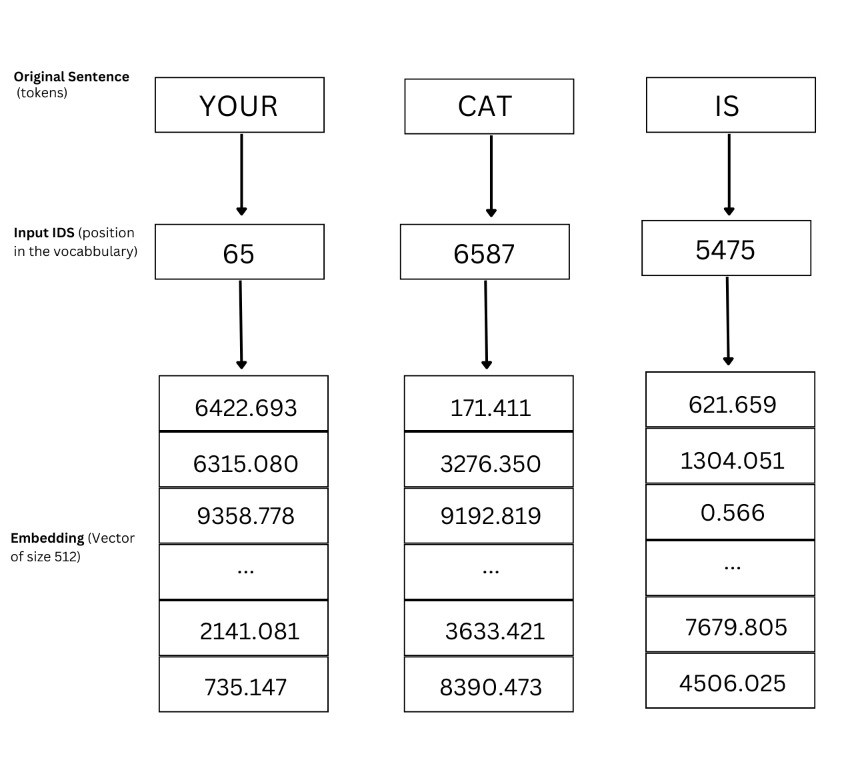
\includegraphics[width=0.65\textwidth]{images/input.jpg}
    \caption{Converting Tokens to Vector Representations}
    \label{fig:input}
\end{figure}
\subsubsection{Positional Encoding}

Once each token is assigned an input id, the vector is fetched from the word embeddings. Each input embedding is then augmented with positional encoding. Positional encoding allows the transformer to understand the sequence of the input tokens. These are calculated using sinusoidal encodings. The figure \ref{fig:sinusoidal} shows how the sinusoidal encodings are generated and the positions are found using three different periods of a sine wave function.
Once the positional encodings are calculated, they are reused and not recomputed. Supposing an example input the sentence "Your Cat Is A Cute Cat". If each word is regarded as a token, then each token receives an input ID that corresponds to the word embedding. The corresponding vectors are fetched and positional encodings are added to them as shown in figure \ref{fig:positional}.
The positional encodings are of the same size as the input. The positional encodings in this example are of the shape (1,512) making it easier to add them up.
\begin{figure}[h]
    \centering
    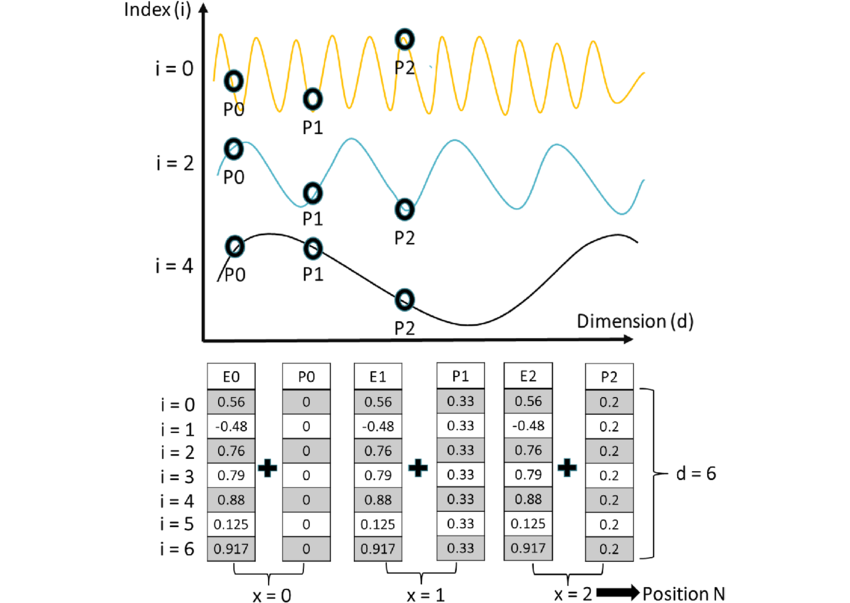
\includegraphics[width=0.65\linewidth]{images/sinusoidal.png}
    \caption{Sinusoidal Positional Encoding}
    \label{fig:sinusoidal}
\end{figure}

\begin{figure}[h]
    \centering
    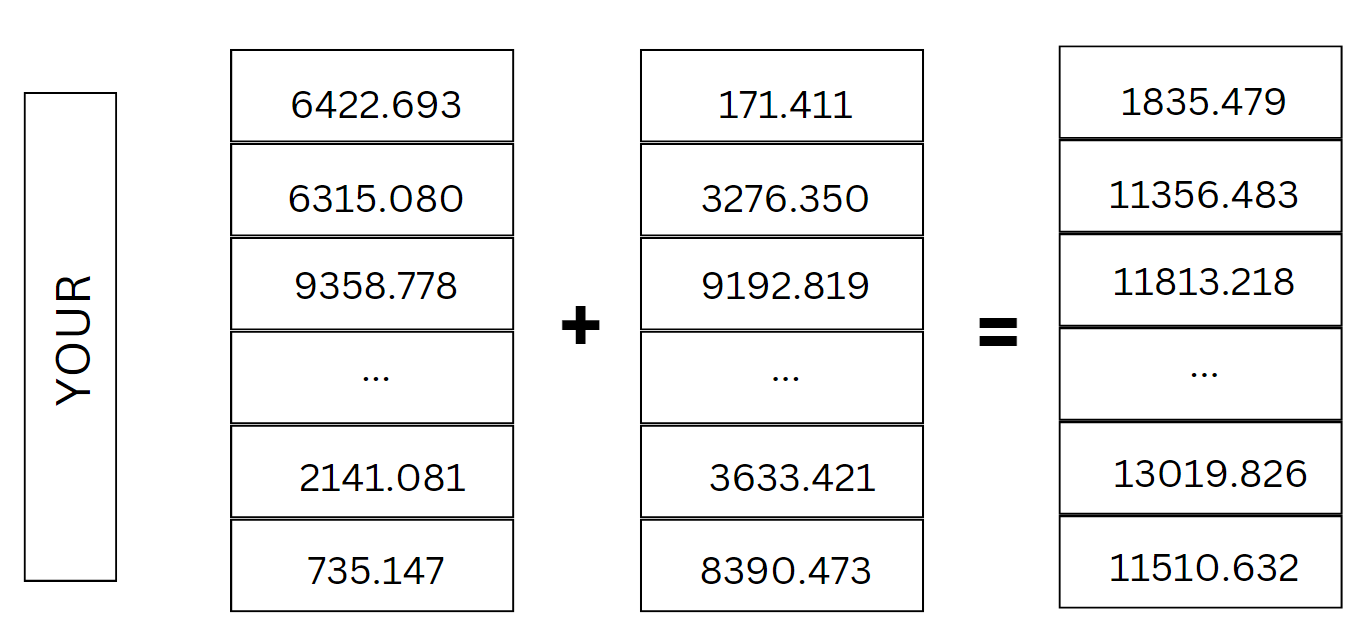
\includegraphics[width=0.75\textwidth]{images/positional.png}
    \caption{Appending Positional Encoding}
    \label{fig:positional}
\end{figure}
\subsubsection{Self-Attention Module}

After augmentation of the input with positional encoding, the vectors are converted into three different projections which are fundamentally three copies. Projection 1 becomes the query, projection 2 becomes the keys, and so projection 3 becomes values. The intuition behind self-attention is to provide each word the required attention from other words. Hence the query is multiplied with the keys to get a matrix. Although additive attention is better at higher values of dk, multiplicative attention is preferred because it computes faster than the additive attention. The multiplicative attention suffers from explosive gradients problem giving extreme values and so a scaling factor of $\sqrt{dk}$ is used. 
\begin{figure}[h]
    \centering
    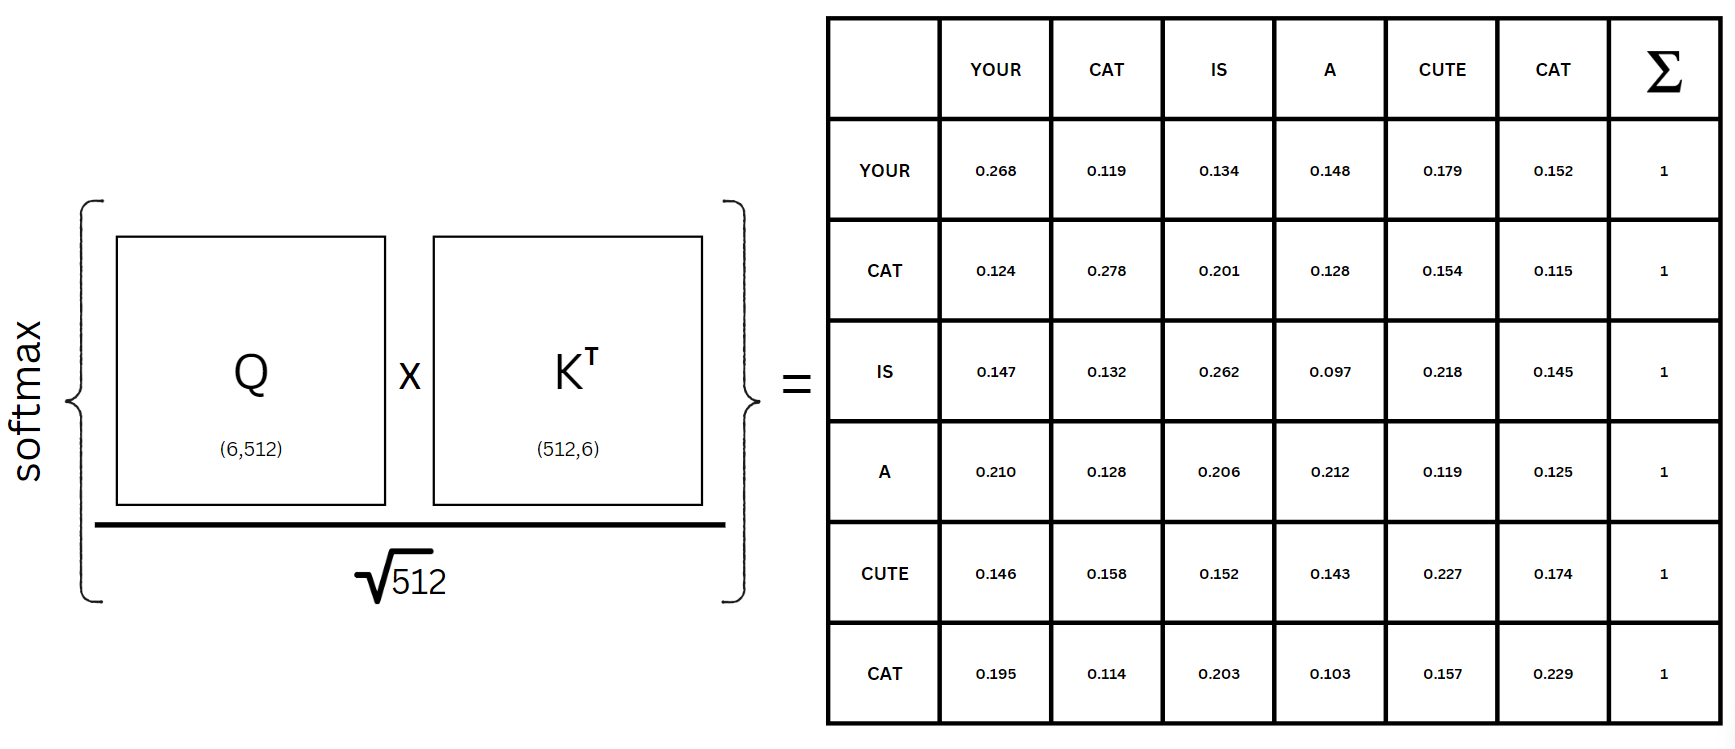
\includegraphics[width=0.75\linewidth]{images/self-attention1.png}
    \caption{Multiplicative Attention}
    \label{fig:self-attention1}
\end{figure}
Conforming to the conventions used in the original paper of transformers by Vaswani et al. 2017, we have mentioned a variable dk. The variable refers to the length of the vector in the word embeddings. Considering the vector shape in the embeddings is of the shape (512,1); then the product of vector of Queries and Keys is divided by the scaling factor of $\sqrt{512}$. 

A product of Values is taken with the output of softmax applied to the previous dot product. The final matrix gives the attention scores. This process as depicted in figures \ref{fig:self-attention1} and \ref{fig:self-attention2} is known as self attention. The input consists of queries and keys of dimension \(d_{k}\), and values of dimension \(d_{v}\). Dot products of the query with all keys, dividing each by the square root of \(d_{k}\), and applying a soft max function to get the weights on the values. The computation of the output matrix is expressed as follows:
\begin{equation}
% \text{Attention}(Q, K, V) = \text{softmax}(\frac{QK^T}{\sqrt{d_k}})V
Attention(Q, K, V ) = softmax\left(\frac{QK^{T}}{\sqrt{d_k}}\right)V
\label{eq:self_attention}
\end{equation}
\begin{figure}[h]
    \centering
    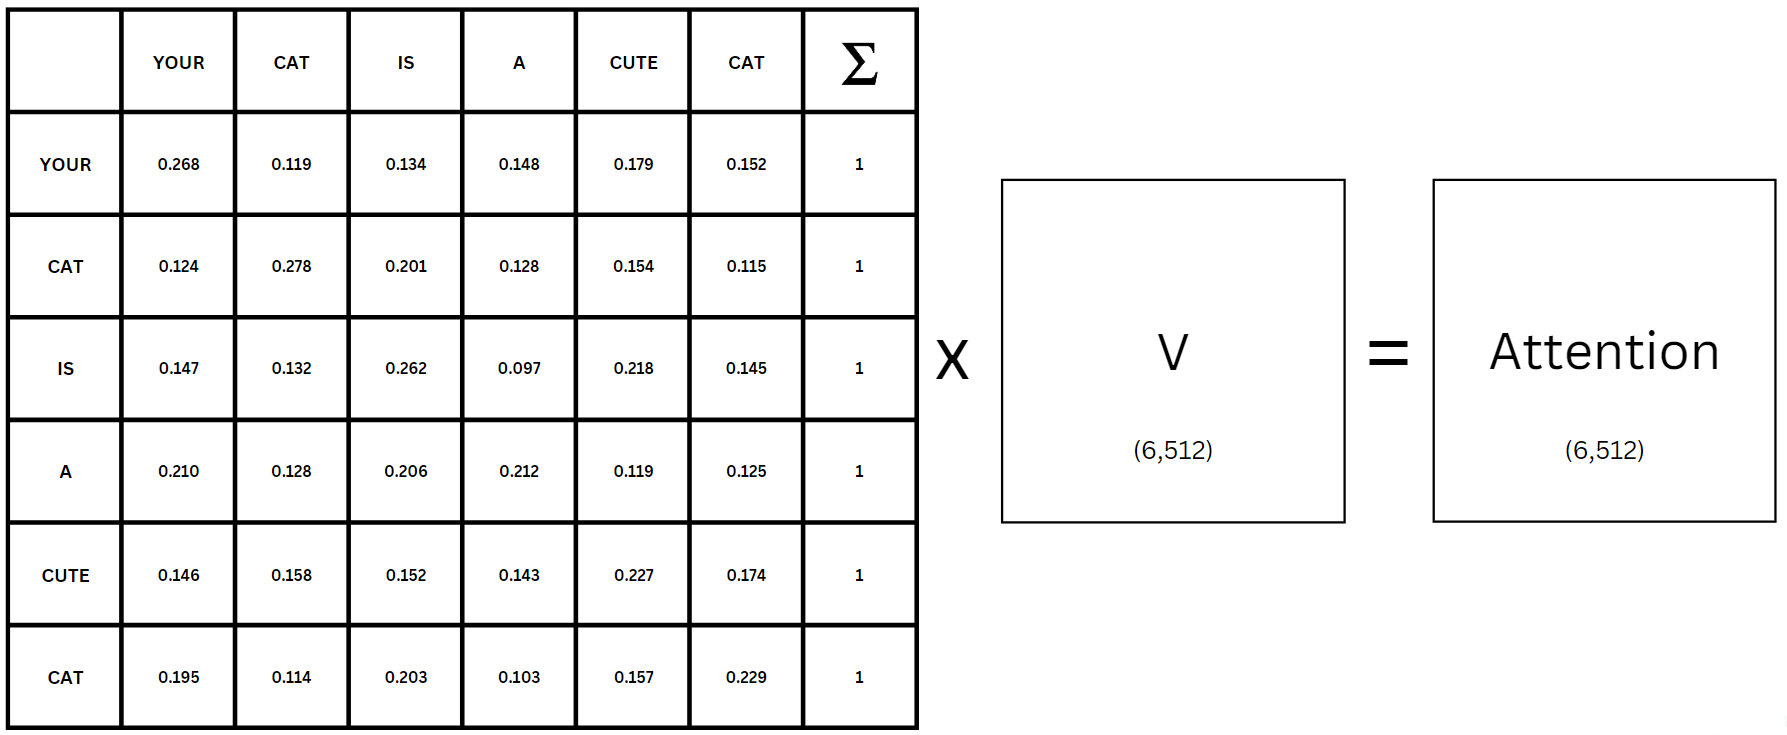
\includegraphics[width=0.75\linewidth]{images/self-attention2.png}
    \caption{Dot Product with Values Gives Attention}
    \label{fig:self-attention2}
\end{figure}
In the example the shape of queries and keys is (6,512). After their dot product, scaling and softmax their shape is (6, 6) which is \((seq, seq)\). A dot product with values of shape (6, 512) returns an attention matrix of shape (6, 512). To make things easier to understand we will be introducing some variables. 6 from the shape of the input is variable \(seq\), hence the number of tokens in the input. \(d_{model}\) is the size of the word embedding which in this case is 512. So the shape of the attention module's output is \((seq, d_{model})\).

\subsubsection{Multi-Head Attention}


To learn different representations, a dot product between each Query, Key and Value is taken with their respective weights. The input matrix is split across the columns according to the number of heads in the self-attention module. The size of the columns now becomes the scaling factor \(d_k\) given by: \[dk = \frac{d_{model}}{h}\]
\begin{figure}[H]
    \centering
    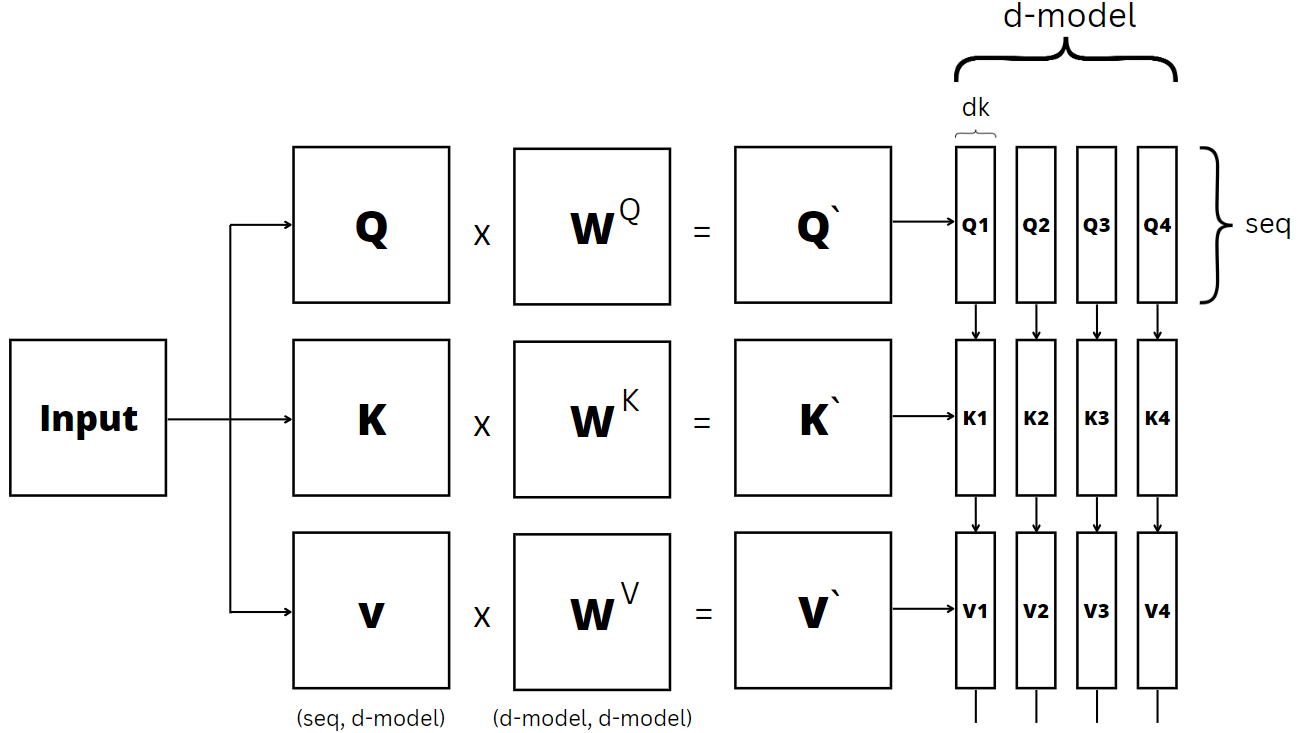
\includegraphics[width=0.75\linewidth]{images/multi1.png}
    \caption{Splitting for Multi-Head Attention}
    \label{fig:multi-head1}
\end{figure}
Then as explained previously, each split is processed by a different attention head. The output of all attention heads are then finally merged and multiplied by weights to give multi-head attention scores. A single head's attention is given as:
\begin{equation}
    head_i = Attention(QW^{Q}_i, KW^{K}_i, VW^{V}_i )
    \label{eq:single-head}
\end{equation}
The Multi-head attention is given as:
\begin{equation}
    MultiHead(Q, K, V) = Concat\left(head_1...head_h\right)W^O
    \label{eq:multi-head}
\end{equation}
Figures \ref{fig:multi-head1}  and \ref{fig:multi-head2} show the complete process involved in multiplicative attention.
\begin{figure}
    \centering
    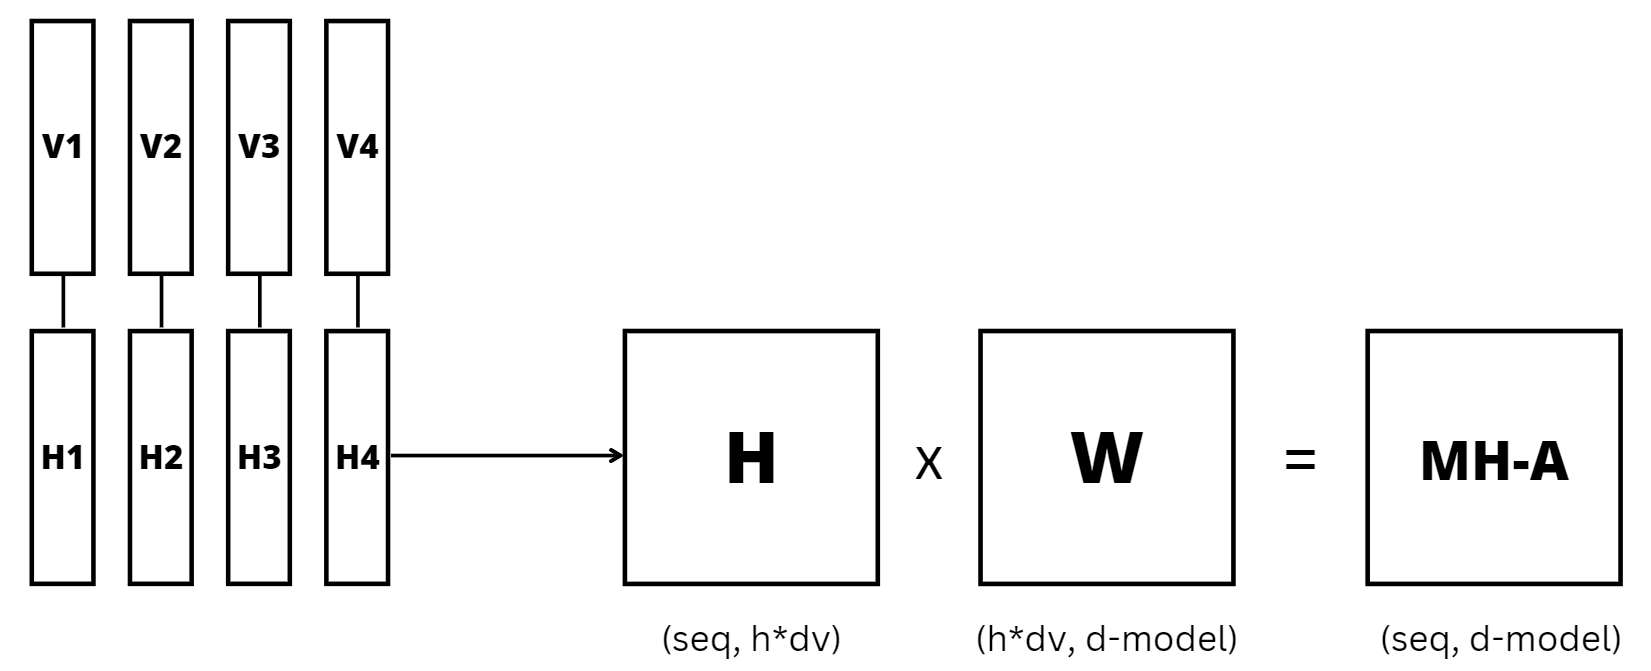
\includegraphics[width=0.75\linewidth]{images/multi-head.png}
    \caption{Output for Multi-Head Attention}
    \label{fig:multi-head2}
\end{figure}
Using the conventions stated before, it can be clearly seen that a dot product is taken for each of the queries, keys and values of shape \((seq, d_{model})\) with their respective weights of shape \((d_{model}, d_{model})\). The dot product gives the output in shape \((seq, d_{model})\) which is then split according to the number of heads \(h\). The shape of \(H\) is defined to be \((seq, h*dv)\) where \(dv\) is the size of values matrix which in this case is equal to \(dk\) but can be kept different. The product with weights of shape \((h*dv, d_{model})\) gives the original shape of \((seq, d_{model})\) which shows \(dv\) can be different from \(dk\).
\subsubsection{Residual Connection}
To keep the original input intact and not lose any important information, an additive attention is used by adding the original input. The output is then batch normalized and passed to the feed-forward neural network. Batch normalization computes the mean and variance across the entire batch for each feature independently normalizing the features within each example based on the statistics of the entire batch. A visual representation of batch normalization is shown in figure \ref{fig:batch-norm}. It is preferred over layer normalization because in time series transformer because it is less affected by the variation in sample lengths found in time series data. The original transformer uses layer normalization to cater to varying input lengths.

\begin{figure}[H]
    \centering
    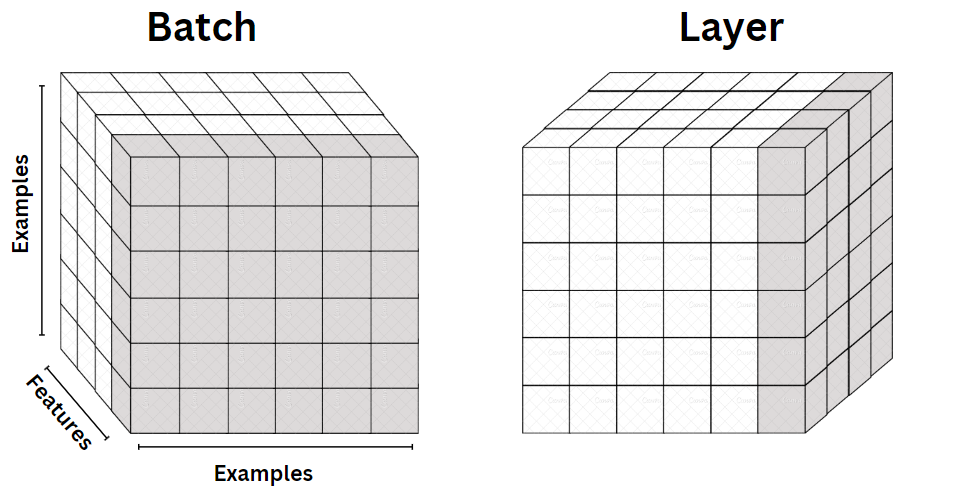
\includegraphics[width=0.7\linewidth]{images/batch-norm.png}
    \caption{Batch Normalization vs Layer Normalization}
    \label{fig:batch-norm}
\end{figure}
\subsubsection{Feed-Forward Neural Network}
The Feed forward neural network uses perceptrons. The perceptrons also known as neurons, compute the dot product of the input with the weights which are initialized using either Xavier Initialization or He Initialization given by: \[W \sim U\left(-\frac{\sqrt{6}}{\sqrt{n_{in}+n_{out}}} ,\frac{\sqrt{6}}{\sqrt{n_{in}+n_{out}}}\right)\]
and
\[W \sim N\left(0 ,\sqrt{\frac{2}{n_{in}}}\right)\]
where U is uniform distribution and N is Normal distribution. An activation function usually Rectified Linear Unit (ReLU) given as: \[ f(x) = \max(0, x) \]
is used on the product and weights are updated using the Adam optimization algorithm. The feed-forward network consists of multiple hidden layers which allow the network to explore the features and relations between tokens in a higher dimensional space. The networks also utilize the concept of auto-encoders where the input is squeezed in a lower dimension and then unsqueezed for effective representation learning. Representation learning refers to learning of underlying structures and relations in the data. Once the representations are learned, they can be used for downstream tasks such as data imputation, regression, classification, and for our case \textbf{forecasting}.

\subsection{Decoder}
The decoder as depicted in figure \ref{fig:decoder} utilizes similar concepts as the encoder. The decoder has two attention modules. The first attention module is called the masked attention module. The input to this module is the output of the transformer's previous pass. In the beginning when there is no output generated, it utilizes a starting terminal character to symbolize the beginning of a sentence. The rest of the output is masked with negative infinity values which prevents the model from knowing the future tokens. This makes the model causal, making it depend on the previously generated token. The masked values when pass through the softmax become 0, hence the name masked attention module. The output of this is used as values and passed along with the output of the encoder which is used as queries and keys in the cross attention module. The output of the cross attention is then passed to feed forward network. The output of the last layer is called logits on which a softmax can be applied but it usually doesnt perform really well. Instead a beam search can be used which selects for each step top B words and evaluate all possible next words for each word selected.
In our use case of forecasting, we will stick to the encoder part because the decoder is more likely used for generative tasks. Using the encoder component only makes the model versatile as it not only helps in regression and classification tasks but can also be used in forecasting.

\begin{figure}[H]
    \centering
    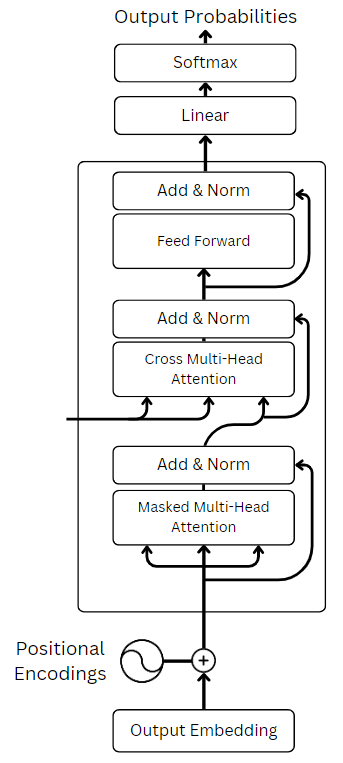
\includegraphics[width=0.35\textwidth]{images/decoder.png}
    \caption{Decoder of a Transformer}
    \label{fig:decoder}
\end{figure}
\subsection{Preprocessing} 
Preprocessing data is a crucial task in time series forecasting. We use simple traditional preprocessing techniques involving scaling to a range of [0,1] or [-1,1], outlier removal, feature engineering, and Input Vector (X) Model Vector (U) Positional Encoding (U') Self Attention Layer Output Vector (Z) standard scaling.
For categorical data, we need to first encode it using Label Encoding i.e., we give a unique numerical value to each category. Once scaling and encoding has been performed, now we bring the sample vectors into the dimensions acceptable by the input. The input format (dimensions) used is an np.ndarray with 3 dimensions i.e., [samples x variables x sequence length]. 
\subsection{Feature Vectors} 
In particular, each training sample  \(X \in R^{w*m}\) where \(w\) is the length of multivariate time series or the number of examples in the input data, and \(m\) is the count of different variables constituting a sequence \(seq\) of \(w\) feature vectors. 
\begin{equation}
    x_{t} \in \mathbb{R}^{m}:X \in \mathbb{R}^{w*m} = [x_{1}, x_{2}, . . ., x_{w}]
    \label{eq:input}
\end{equation}

\subsection{Model Vector (U)}
The figure \ref{fig:base-model} shows the encoder part of the transformer being used in forecasting. The original feature vectors \(x_{t}\) are first normalized by subtracting the mean and dividing by the variance across the training set samples, and then linearly projected onto a \(d\) dimensional vector space, where \(d\) is the dimension of the transformer model sequence element representations, \(d_{model}\): 
\begin{equation}
    u_{t} = W_{p}\cdot x_{t} + b_{p}
    \label{eq:linear projection}
\end{equation}
where \(W_{p} \in \mathbb{R}^{d*m}, b_{p} \in \mathbb{R}^{d}\) are learnable parameters and \(u_{t} \in \mathbb{R}^{d}, t = 0, …, w\)  are the model input vectors, which correspond to the word vectors of the NLP transformer. So a combined form is given by:
\begin{equation}
    U = X \cdot W_{p}^\textit{T} + b_{p}
\end{equation}
These will become the queries, keys, and values of the self-attention layer, after adding the positional encoding and multiplying by the corresponding matrices.
\begin{figure}[h]
    \centering
    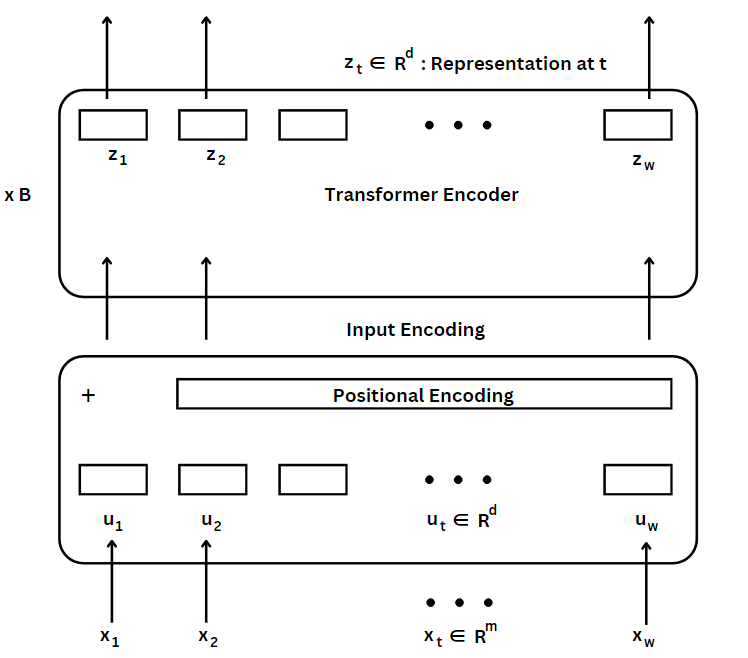
\includegraphics[width=0.7\textwidth]{images/base_tst_model.png}
    \caption{Base Model Representing Transformer}
    \label{fig:base-model}
\end{figure}
\subsection{Positional Encoding}
Before sending the model input vector (U) to the self-attention layer, positional encoding is added to the feed-forward architecture to make it aware of the sequential nature of the time series data. Unlike the original transformer's fixed sinusoidal encodings, fully learnable positional encodings are used. The model’s performance shows that it is independent of the added positional embedding because both the numerical time series information and positional encoding are orthogonal to each other in the vector dimensional space. The positional encodings given by:         \(W_{pos} \in \mathbb{R}^{w*d}\) are added to the input:
\begin{equation}
    U \in \mathbb{R}^{w*d} = [u_1...u_w] : U' = U + W_{pos}
    \label{eq:positional-encoding}
\end{equation}
The dimensions of the input are now \((seq, d_{model})\)
\subsection{Variation in data} 
Time series data may show inconsistency in its length. The shorter samples in the input are padded with arbitrary values and a padding mask adds large negative values to the arbitrary paddings forcing the model to ignore padded positions in softmax and allow parallel processing.

\subsection{Forecasting}
The base model architecture discussed above can be used for the purposes of regression, classification, and forecasting with the following modification: the final representation vectors \(z_{t}\in \mathbb{R}^{d}\) corresponding to all time steps are concatenated into a single vector \(Z \in R^{d*w} = [z1;…;zw]\) , which serves as the input to a linear output layer with parameters \(W_{o} \in \mathbb{R}^{n×(d \cdot w)} , b_{o} \in \mathbb{R}^{n}\)  , where \(n\)  is the number of scalars to be estimated for the regression problem (typically  \(n\)=1), or the number of classes for the classification problem:
\begin{equation}
    \hat{y} =W_{o}Z+b_{o}
\end{equation}
In the case of regression, the loss for a single data sample will simply be the squared error: 
\begin{equation}
    L=|\hat{y}-y|^{2}
\end{equation} 
Where, \(y \in \mathbb{R}^n\)  is the ground truth values. We need to provide different masking patterns to the regression problem that helps in predicting the future values. We may use a sliding window and decide a horizon to predict the future values. 

\section{Experimental Setup}
\subsection{Data Source}
The Data that needs to be collected is obtained from:
\begin{itemize}
    \item Nurse Surveys: The on-duty nurses are asked questions regarding the duties they perform for each patient and how these duties differ for each patient.
    \item Observations recorded from a hospital visit
    \item Research Papers: Using previous research that has been done on electronic nursing systems to extract key information about the nursing workflow.
    \item CCTV Footage: Cameras are setup to collect data which is used to train the model.
\end{itemize}
\subsection{Data Collection Methodology}
The footage is taken from the cameras installed in the wards. Multiple RGB cameras are set up in a ward depending on the size of the ward and the arrangement of the beds. The Cameras captures and detects the patient lying on the bed and the data from the machines next to the patient. To cover all the patients in the ward, cameras facing both sides of the ward will be installed.\\
The footage is cleaned to remove redundant data or parts of the video that are empty. The footage divided into training and testing datasets is used to train and test the AI Model. A clear image of patient vitals monitor is also taken to train the model on different interfaces. 
Surveys are conducted to list down all the details of tasks assigned to a nurse. The patient records maintained by the nurse are studied thoroughly to extract any missed information logged in the records. Previous researches on ENS are used to extract information that is required by a doctor. During the time spent in the nursing ward, observations will be noted about the details involved in nursing. 
Data will be obtained from atleast 4 different hospitals.

\subsection{Data Processing Procedures}
Redundant data and any part of the video that is noisy is removed. The video contains hours of unnecessary stream where there is no one in the ward are trimmed away. Once the necessary processing is done, the video is used for training the AI model.\\
To cater the usage rights and privacy concerns, features are extracted such as patient face. Once the features from this frame are extracted, the video is blurred or have a filter added to it.
The features extracted from this clip are sent down with the video. The video is not sent as a whole because it requires a huge bandwidth so the video is compressed and then sent to the cloud for further processing. The AI Model that has already been trained, utilizes the incoming data and extract the necessary features to classify activities and extract vitals. The model then sends a signal to the dashboard and mobile application alerting the caretakers.\\
The data collected from surveys, interviews, and previous research is used to refine the features of the cross-platform ENS solution.

\subsection{Data Storage and Security}
The video is processed on the desktop at the user’s own end to ensure data integrity. The data extracted from the video is encrypted before being sent to the cloud server to prevent breach of privacy and confidentiality. Once the data is processed in the cloud, it is discarded. The information extracted is stored in an encrypted format. An MOU which has been signed will act as a form of undertaking; that the members working on this project will comply to the data usage rights prescribed by the hospital and will maintain the code of ethics while delivering the necessary output.

% Write in your own chapter title to set the page header